\appendix

\chapter{TUNING THE TIMING SYNCHRONIZER}
\label{app:tuning}

\section{The requirement of tuning}

The timing synchronizer is makes several assumptions about the system in
question, and these assumptions are coded in the form of numerical parameters.
The values of these parameters must be determined empirically, by performing a
few measurements on the system. The `system', here, refers to the
transmitter-channel-receiver setup.

One possible use case scenario for tuning may be as follows: the synchronizer
is currently tuned for some frequency, but we desire to change the frequency of
operation by a large value. As a result, the expected degree of noise in the
system may increase. This could, potentially, cause erroneous packet detection
in a noisy patch, or more likely, cause a good packet to get dropped.

It is good to always keep a check on how many packets are being received, and
whether the rate at which they are being detected is equal to the rate at which
they are being transmitted. If it is found that the rate of reception of
packets is significantly lower, it is likely that the synchronizer needs to be
tuned.

%%%%%%%%%%%%%%%%%%%%%%%%%%%%%%%%%%%%%%%%%%%%%%%%%%%%%%%%%%%%%%%%%%%%%%%%%%%%%%%

\section{The debug files}

To run the program with debugging enabled for the timing synchronizer, clean
and re-compile the program with the make option \verb!DEBUG_TIMING_SYNC=true!
set, like so:
\lstset{language=}
\begin{lstlisting}
	$ make clean
	$ make cleandata
	$ make DEBUG_TIMING_SYNC=true
\end{lstlisting}
\lstset{language=C++}

Then, run the transmitter and receiver as usual, with the desired parameters,
for a short period of time. At the receiver end, the timing synchronizer should
output a bunch of \texttt{.out} files. Each of these is a binary file of
128-bit complex numbers, composed of two \lstinline!double!s. A list of these
files and descriptions of their content follows.

\begin{description}
	\item[\texttt{input\_data.out}] \hfill \\
		This file contains the received data stream as seen by the timing
		synchronizer. Only parts of frames, which are discarded once found (as
		described in subsection~\ref{subsec:frame-discard}), may be visible.
		Specifically, only the first half of the two-frame block is saved into
		this file. If a frame was found in the first half, then the parts of it
		that go into the second half are never `seen' by the timing
		synchronizer once the frame is discarded. \\
		All other debug files also share this particular property. Therefore,
		all debug files are of the same length, and their data can be overlaid
		on a plot (such as in figure~\ref{fig:metric}).
	\item[\texttt{abs.out}] \hfill \\
		This file contains the absolute value of the cross-correlation and the
		product of the autocorrelations of the correlation windows. The
		absolute value of the cross-correlation is stored in the real part of
		the data and the product of the autocorrelations is stored in the
		imaginary part of the data. For data location $i$, the two correlation
		windows start \emph{at} $i$ and extend $2n-1$ locations to its right.
	\item[\texttt{found\_packets.out}] \hfill \\
		This file contains the points where packets were found. If a packet
		was found at a given location, then this file contains a 1 at that
		position. At all other locations, it contains 0. \\
		While using 128-bit complex numbers may seem like a waste of space, it
		is convenient since it enables one to use the same mechanism to read
		all the debug files, as opposed to having to remember what number
		format needs to be used in each case.
	\item[\texttt{left\_avg\_new.out}] \hfill \\
		This contains the average, $\bar{x}$ of the left correlation window, as
		computed using the running average algorithm.
	\item[\texttt{right\_avg\_new.out}] \hfill \\
		This contains the average, $\bar{y}$ of the right correlation window,
		as computed using the running average algorithm.
	\item[\texttt{fine\_metric.out}] \hfill \\
		This contains the value of the fine metric (refer
		subsection~\ref{subsec:fine-metric}), wherever it had to be computed.
		At other locations, it contains 0.
\end{description}

%%%%%%%%%%%%%%%%%%%%%%%%%%%%%%%%%%%%%%%%%%%%%%%%%%%%%%%%%%%%%%%%%%%%%%%%%%%%%%%

\section{Performing tuning}

Check whether tuning is required by overlaying the input data, the metric and
the positions of found packets on a plot. In python, with the packages numpy
and matplotlib installed, this can be achieved as follows:

\lstset{language=Python}
\begin{lstlisting}
	import numpy as np
	import matplotlib.pyplot as plt

	a = np.fromfile('input_data.out', dtype=np.complex128)
	b = np.fromfile('abs.out', dtype=np.complex128)
	f = np.fromfile('found_packets.out', dtype=np.complex128)
	m = b.real / b.imag
	m = np.where(np.isfinite(m), m, np.zeros(m.size))
	
	plt.plot(abs(a), 'k')
	plt.plot(m)
	plt.plot(f.real)
	plt.show()
\end{lstlisting}
\lstset{language=C++}

\begin{figure}[h]
	\centering
	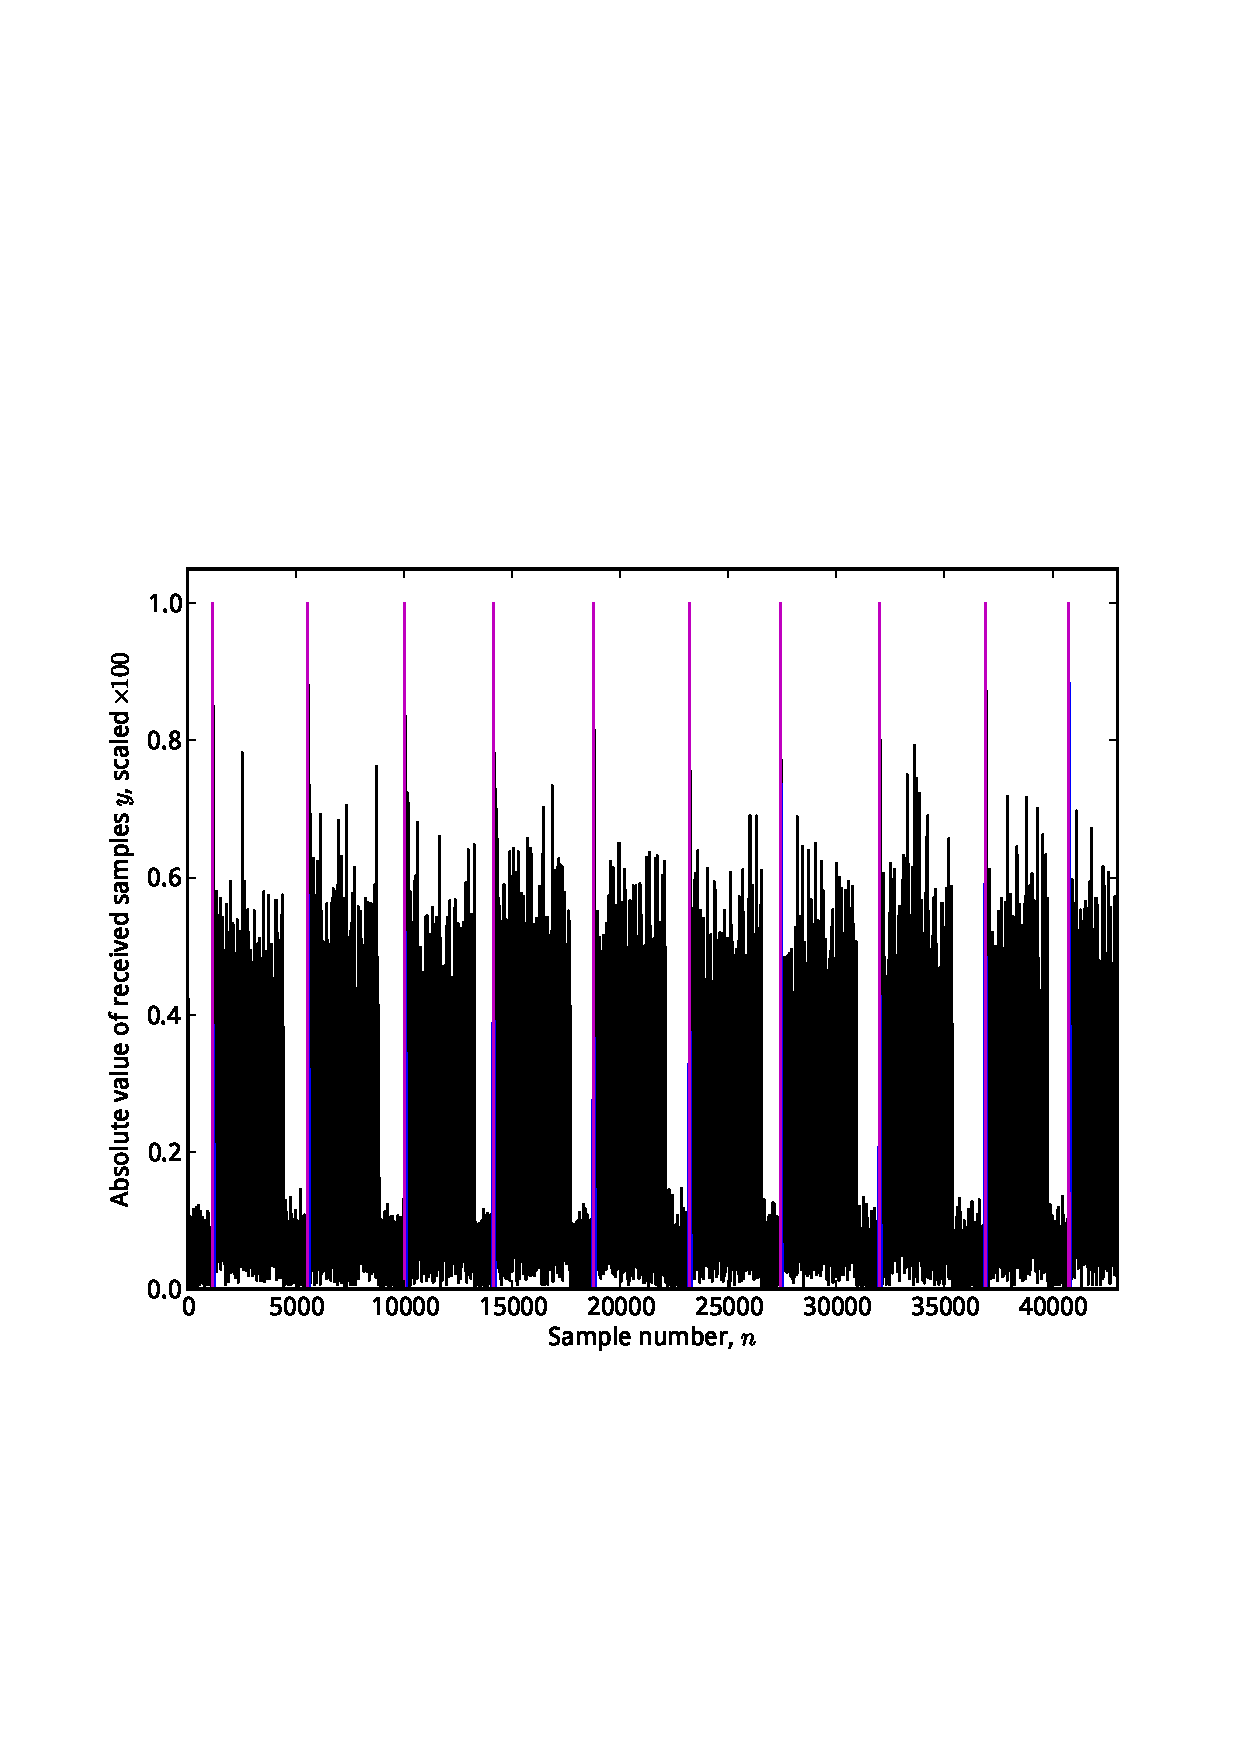
\includegraphics[width=0.8\textwidth]{packets}
	\caption{Packet stream after passing through the timing synchronizer}
	\label{fig:packets}
\end{figure}

This should, after suitable scaling, give a plot such as the one in
figure~\ref{fig:packets}. Note that all packets have been detected, as
indicated by the presence of the magenta line.

If there are several places where the packet fails to be detected, however,
then it calls for checking whether or not the metric exceeds the threshold. If
not, then the \lstinline!PACKET_THRESHOLD! parameter in the
\texttt{parameters.h} file needs to be changed so that the threshold is crossed
by the metric at the starting point of every packet, but is \emph{not} crossed
in other random locations.

Similarly, there may also be a need to modify the \lstinline!FINE_THRESHOLD!
parameter in the same file.

Furthermore, if the noise variance of the channel is high, it is possible for
the absolute value of the cross-correlation of noise to go above the
\lstinline!CROSS_CORR_THRESHOLD!. This may result in undesired effects, as
described in subsection~\ref{subsec:cross-corr-threshold}. Such a case can be
identified because the metric will be visible even in regions where there is no
packet.

In this case, plot the absolute value of the cross-correlation (the real part
of the data from the \texttt{abs.out} file) and overlay it on the data stream.
It should now be possible to set the \lstinline!CROSS_CORR_THRESHOLD! at a
value such that it is higher than the absolute value of the cross-correlation
of noise, but lower than the absolute value of cross-correlation of parts of a
packet.
